% TODO Circuit pic
Two resistor values need to be determined in order ot properly design the differential amplifier.
$R_{REF}$ needs to be determined to design the current source.
The two transistors $M_{2A}$ and $M_{2B}$ are matched and conduct a total current of $I_{SS}$.
Thus, each conducts a current of $\frac{I_{SS}}{2}$.
Because $M_{D}$ is diode connected, $V_{DS} = V_{GS}$.
Therefore, $R_{REF}$ can be determined using Ohm's Law:

\begin{equation}
	\label{eq:r_ref}
	R_{REF} = \frac{ V_{DD} - V_{GS} }{ \frac{I_{SS}}{2} }
\end{equation}

Ignoring channel-length modulation effects, the current through $M_{D}$ can be acquired using $\frac{k_{n}'}{2} \frac{W}{L} ( V_{GS} - V_{tn} )^{2} = \frac{ I_{SS} }{ 2 }$.
Therefore, $V_{GS}$ can acquired using:

\begin{equation}
	\label{eq:vgs}
	V_{GS} = V_{tn} + \sqrt{\frac{ I_{SS} }{ k_{n}' \frac{W}{L} }}
\end{equation}

Using equations (\ref{eq:vgs}) and (\ref{eq:r_ref}), $R_{REF} = $ \rref.
This ensures that the $I_{SS} = $\iss specification is met.
To achieve maximum output swing, one must know the midpoint of $V_{out}^{+}$ and $V_{out}^{-}$, referred to as $V_{midpoint}$.
From this information, $R_{D}$ can be acquired:

\begin{equation}
	\label{eq:r_d}
	R_{D} = \frac{ V_{DD} - V_{midpoint} }{ \frac{ I_{SS} }{ 2 } }
\end{equation}

$V_{midpoint}$ is the only unknown for this circuit.
At either $V_{out}^{+}$ or $V_{out}^{-}$, the highest value is the supply voltage $V_{DD}$ when the transistors are cutoff.
The lowest value is approximately the output voltage during the transition from triode to saturation.
This occurs when $V_{DS} = V_{GS} - V_{tn}$ or equivalently when $V_{D} = V_{out}^{+,-} = V_{G} - V_{tn}$.
The transistor is biased at $V_{G} = $ \vbias and $V_{tn}$ is known.
Therefore, the midpoint of the output voltage at either side of the amplifier occurs at:

\begin{equation}
	\label{eq:v_midpoint}
	V_{midpoint} = \frac{ V_{High} + V_{Low} }{ 2 } = \frac{ V_{DD} + ( V_{G} - V_{tn} ) }{ 2 }
\end{equation}

Using equations (\ref{eq:r_d}) and (\ref{eq:v_midpoint}), $V_{midpoint} = $\vmidpoint and $R_{D} =$\rd .
Figure (\ref{fig:diff_amp}) depicts the amplifier design with the DC operating point results.

\FloatBarrier

\begin{figure}[h!]
	\centering
	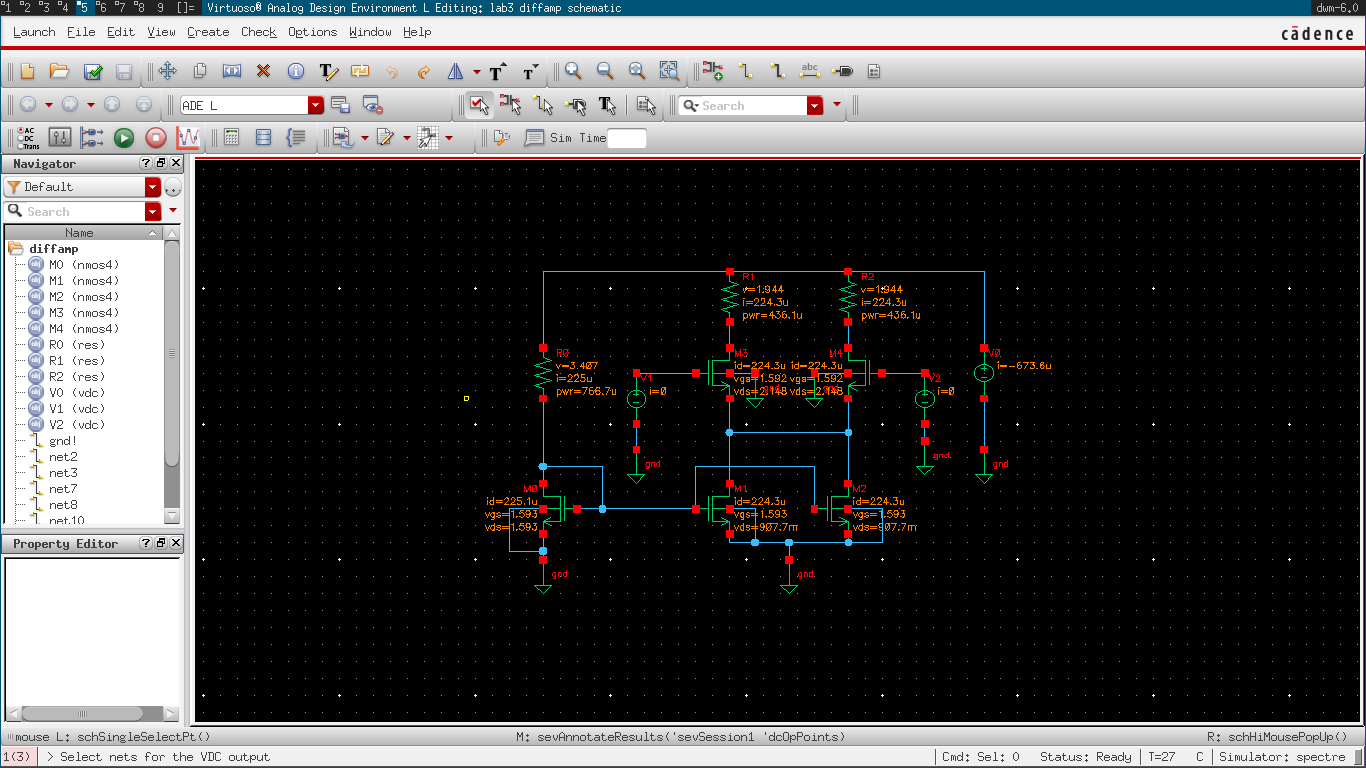
\includegraphics[scale=0.75]{../images/diff_amp.PNG}
	\caption{Differential Amplifier with DC Operating Point Results}
	\label{fig:diff_amp}
\end{figure}

\FloatBarrier

All of the transistors are in saturation as expected.
$I_{SS}$ is about $448.6$\si{\micro\ampere}, which is slightly below the desired $450$\si{\micro\ampere}.
This is a result of channel-length modulation effects causing the currents in the current source to depend on $V_{DS}$.
Let $V_{DS,D}$ be $V_{DS}$ for $M_{D}$ and $V_{DS,AB}$ be $V_{DS}$ for either $M_{2A}$ or $M_{2B}$.
To a first order approximation, the ratio of the current in $M_{2A}$ or $M_{2B}$ to the current in $M_{D}$ is:

\begin{equation}
	\label{eq:ratio}
	\frac{ 1 + \lambda _{n} V_{DS,AB} }{ 1 + \lambda _{n} V_{DS,D} }
\end{equation}

If the current through $M_{D}$ as well as other relevant parameters from figure (\ref{fig:diff_amp}) and the MOSFET model are used, then the expected current through $M_{2A}$ or $M_{2B}$ is about $224.3$\si{\micro\ampere}, which is precisely what is observed in the simulation.
If $R_{REF}$ is decreased slightly to $15.09$\si{\kilo\ohm}, $I_{SS}$ becomes exactly $450$\si{\micro\ampere}, determined from the sum of the currents through each current source.
Figure (\ref{fig:diff_amp_2}) depicts the results for this second design iteration.
It should be noted that this does not affect the output voltage swing since that is determined by $R_{D}$.
Furthermore, all of the transistors remain in saturation.

\FloatBarrier

\begin{figure}[h!]
	\centering
	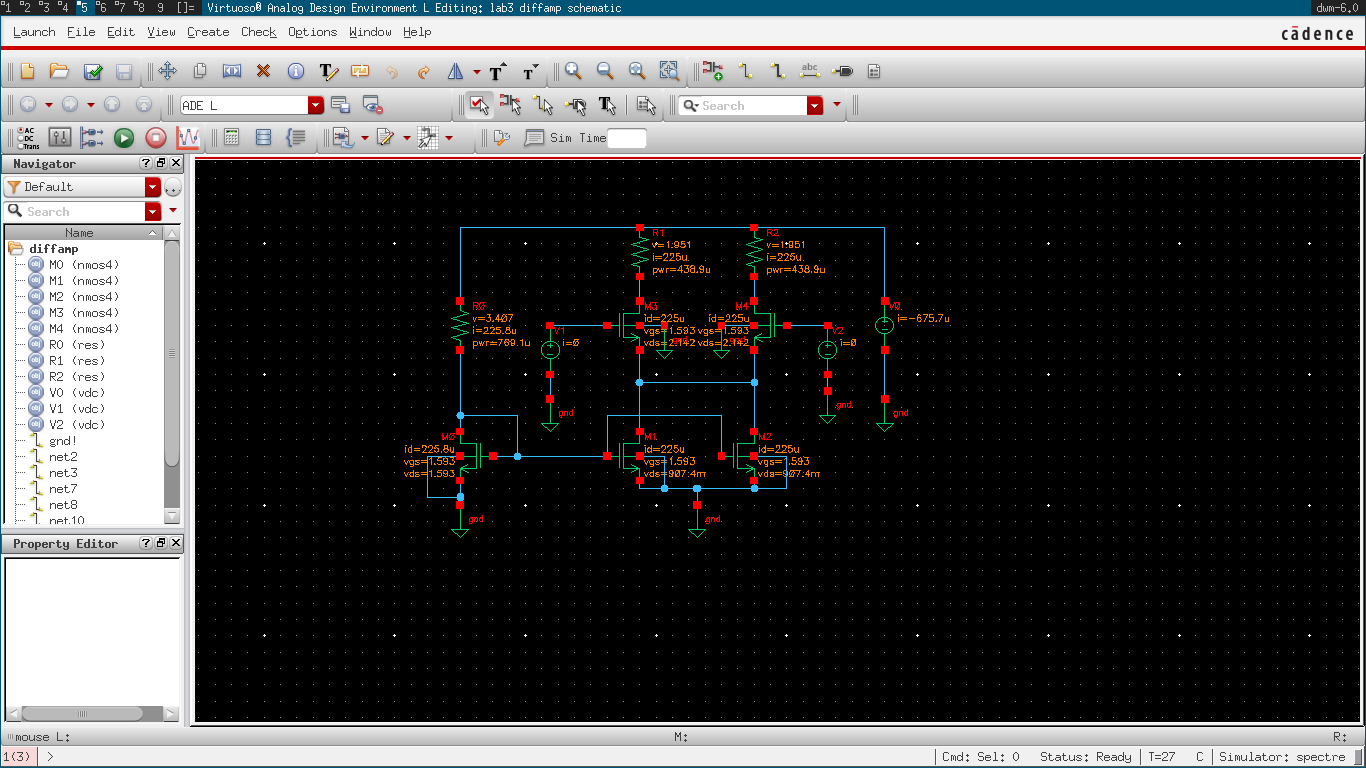
\includegraphics[scale=0.75]{../images/diff_amp_2.PNG}
	\caption{Second Differential Amplifier Design Iteration}
	\label{fig:diff_amp_2}
\end{figure}

\FloatBarrier

Assume the small-signal parameters of the circuit are known.
For only differential mode signals, the source of $M_{1A}$ and $M_{1B}$ becomes an AC ground.
Therefore, the half-circuit is simply a common-source amplifier with drain resistor $R_{D}$.
The negative sign disappears since the negative and positive differential inputs are flipped in the circuit.
$g_{m1A,B}$ is $g_{m}$ for both $M_{1A}$ and $M_{1B}$ which turns out to be the same.
$r_{o1A,B}$ is the output resistance of $M_{1A}$ and $M_{1B}$.

\begin{equation}
	\label{eq:dm_gain}
	A_{dm} = g_{m1A,B} ( R_{D} || r_{o1A,B} )
\end{equation}

The common-mode gain can be acquired by recognizing that the current sources act as MOSFETs with the gate and source grounded since only DC signals exist in the reference part of the circuit.
So, the small-signal model of these transistors reduces to the output resistance of each of the MOSFETs, which turn out to be identical.
$r_{o2A,B}$ is the output resistance of $M_{2A}$ and $M_{2B}$.
Note that $r_{o1A,B} = r_{o2A,B}$.
By analyzing the half-circuit with Kirchhoff's Laws, the following expression is acquired for the common-mode gain:

\begin{equation}
	\label{eq:cm_gain}
	A_{cm} = - \frac{ g_{m1A,B} R_{D} }{ 3 + g_{m1A,B} r_{o1A,B} }
\end{equation}

$g_{m}$ can be calculated using $\frac{ 2 I_{D}' }{ V_{GS} - V_{tn} }$, where $I_{D}'$ is the drain current excluding channel-length modulation effects.
Here, assume $I_{D} \approx I_{D}'$ since channel-length modulation effects are negligible.
$r_{o}$ can be calculated using $\frac{1}{\lambda _{n} I_{D}' }$.
It should be noted that these gain calculations use the values in figure (\ref{fig:diff_amp_2}).

\FloatBarrier

\begin{table}[h!]
	\centering
	\caption{Gains for Part $1$ Second Iteration Amplifier}
	\label{tab:sim1_gain}
	\csvautotabular{../tables/sim1_gain.csv}
\end{table}

\FloatBarrier
